% -------------------------------------------------------------------------------------------------
%
%  Skeleton for semester and master thesis reports at the Laboratory for Software Technology.
%  Based on the skeleton provided by the Institute of Robotics and Intelligent Systems.
%
% -------------------------------------------------------------------------------------------------
%
% USAGE:      compile with PDFLaTeX
%
% HISTORY:    - written by Sascha A. Stoeter <stoeter@iris.ethz.ch>, www.stoeter.com, 02.06.2004
%             - modified by Martin Probst, 18.08.2004
%             - extended and adapted for use at LST by Oliver Trachsel, 2007-08-21
% -------------------------------------------------------------------------------------------------
\documentclass[11pt,a4paper]{book}
\usepackage{lstreport}

% -------------------------------------------------------------------------------------------------
% Add needed packages. Some generally useful packages are listed for
% your convenience.
% -------------------------------------------------------------------------------------------------
\usepackage{subfigure}                          % enable the use of subfigures
\usepackage[thickspace,thinqspace]{SIunits}     %
\usepackage[plainpages=false,pdfpagelabels]{hyperref}    % enable hyperlinks in pdf/ps Docs
\usepackage{listings}                           % to embed source code


% UTF8
\usepackage[utf8x]{inputenc} 

% -------------------------------------------------------------------------------------------------
% Select type of thesis
% -------------------------------------------------------------------------------------------------
\renewcommand{\thesistype}{Bachelor}
%\renewcommand{\thesistype}{Diploma}
%\renewcommand{\thesistype}{Master}

% -------------------------------------------------------------------------------------------------
% Set names
% -------------------------------------------------------------------------------------------------
\renewcommand{\thesisauthor}{Marcel Mohler}
\renewcommand{\thesisadvisor}{Zoltán Majó \\ Tobias Hartmann}

%OWN STUFF###############################################################
\usepackage[english]{babel}

% colors
%\definecolor{orange}{rgb}{1,0.5,0}

% Disable single lines at the start of a paragraph (Schusterjungen)

\clubpenalty = 10000

% Disable single lines at the end of a paragraph (Hurenkinder)

\widowpenalty = 10000
\displaywidowpenalty = 10000
 
% allows for colored, easy-to-find todos

\newcommand{\todo}[1]{\textsf{\textbf{\textcolor{orange}{[[TODO: #1]]}}}}


%##########################################################################


% -------------------------------------------------------------------------------------------------
% Beginning of the main document body
% -------------------------------------------------------------------------------------------------
\begin{document}

% include all bibtex even if not cited
\nocite{*}

% -------------------------------------------------------------------------------------------------
% Front matter with title page, table of contents, and abstracts 
% -------------------------------------------------------------------------------------------------
\frontmatter

% Title page: set title and date 
\thesistitlepage{Profile Caching for the\\Java Virtual Machine
}{August 2015}

% Abstract must not be longer than one page per language. English and
% German abstracts are mandatory.
\chapter*{Introduction}
\label{c:Introduction}
Virtual machines (VMs) like the Java Virtual Machine (JVM) are used as the execution environment of choice for many modern programming languages. 
VMs interpret a suitable intermediate language (e.g., Java Byte Code for the JVM) and provide the runtime system for application programs. VMs usually include a garbage collector, a thread scheduler, and interfaces to the host operating system. 
As interpretation of intermediate code is time-consuming, VMs usually include a \textit{Just-in-time} (JIT) compiler that translates frequently-executed functions or methods to \textit{native} machine code.
\\\\
The JIT compiler executes in parallel to a program's interpretation by the VM and, as a result, compilation speed is a critical issue in the design of a JIT compiler.
Unfortunately, it is difficult to design a compiler such that the compiler produces good or excellent code while limiting the resource demands of this compiler. The compiler requires storage, CPU cycles and even on a multi-core processor, compilation may slow down the execution of the application program.
\\\\
Consequently, most VMs adopt a multi-tier compilation system.
%The first tier usually is the interpretation of a method. If this method is executed frequently, the Tier-1 compiler translates this method into native code.
%The Tier-1 compiler implements only a small set of the know optimization techniques and as result, it had good compilation speed but the generated code is far from the output of an optimizing compiler. Such a compiler is usually the Tier-2 compiler, which takes a longer amount of time and produces optimized native code. To determine which methods should be compiled by the Tier-1 (or Tier-2) compiler, the VM profiles the execution of all application programs to identify “hot” methods.
At program startup, all methods are interpreted by the virtual machine (execution at Tier 0). The interpreter gathers execution statistics called \textit{profiles} and if a method is determined to be executed frequently, this method is then compiled by the Tier 1 compiler. Methods compiled to Tier 1 are then profiled further and based on these profiling information, some methods are eventually compiled at higher tiers.
One of the drawbacks of this setup is that for all programs, all methods start in Tier 0, with interpretation and profiling by the VM. However, for many programs the set of the most used methods does not change from one execution to another and there is no reason to gather profiling information again. 
\\\\
The main idea of this thesis is to cache these profiles from a prior execution to be used in further runs of the same program. 
Having these \textit{cached profiles} available avoids the JIT compiler to gather the same profiling information again. As well as allow the compiler to use more sophisticated profiles early in program execution and prevent recompilations when more information about the method is available. While this in general should not significantly influence the peak performance of the program, the hope is to decrease the time the JVM needs to achieve it, the so called \textit{warmup}.
\\\\
This thesis proposes a design and an implementation of a profile caching feature for \textit{HotSpot}, an open source Java virtual machine maintained and distributed by Oracle Corporation as well as a profound performance analysis using state-of-the-art benchmarks.


%\chapter*{Zusammenfassung}
%Kurzfassung der Arbeit.

% Table of contents
\tableofcontents

% -------------------------------------------------------------------------------------------------
% Main document body
% -------------------------------------------------------------------------------------------------
\mainmatter
\chapter{Motivation}
\label{c:motivation}
I continue with presenting two very simple example methods that illustrate the motivation and benefit from using cached profiles.
This should provide the reader with an understanding how and why cached profiles can be beneficial for the performance of a Java Virtual Machine.
I will omit any implementation details on purpose as they will be discussed in Chapter \ref{c:implementation} in detail.
\\\\
Ideally, being able to reuse the profiles from previous runs should result in two main advantages:
\begin{enumerate}
  \item \textbf{Lower start-up time of the JVM:} Having information about the program flow already, the compiler can avoid gathering profiles and compile methods earlier and directly at higher compilation levels.
  \item \textbf{Less Deoptimizations:} Since cache profiles get dumped at the end of a compilation, when using these profiles the compiler can already include all optimizations for all different method executions. Less uncommon traps need to be placed and less deoptimizations occur.
\end{enumerate}
\begin{figure}[ht]
  \begin{center}
    \centering
    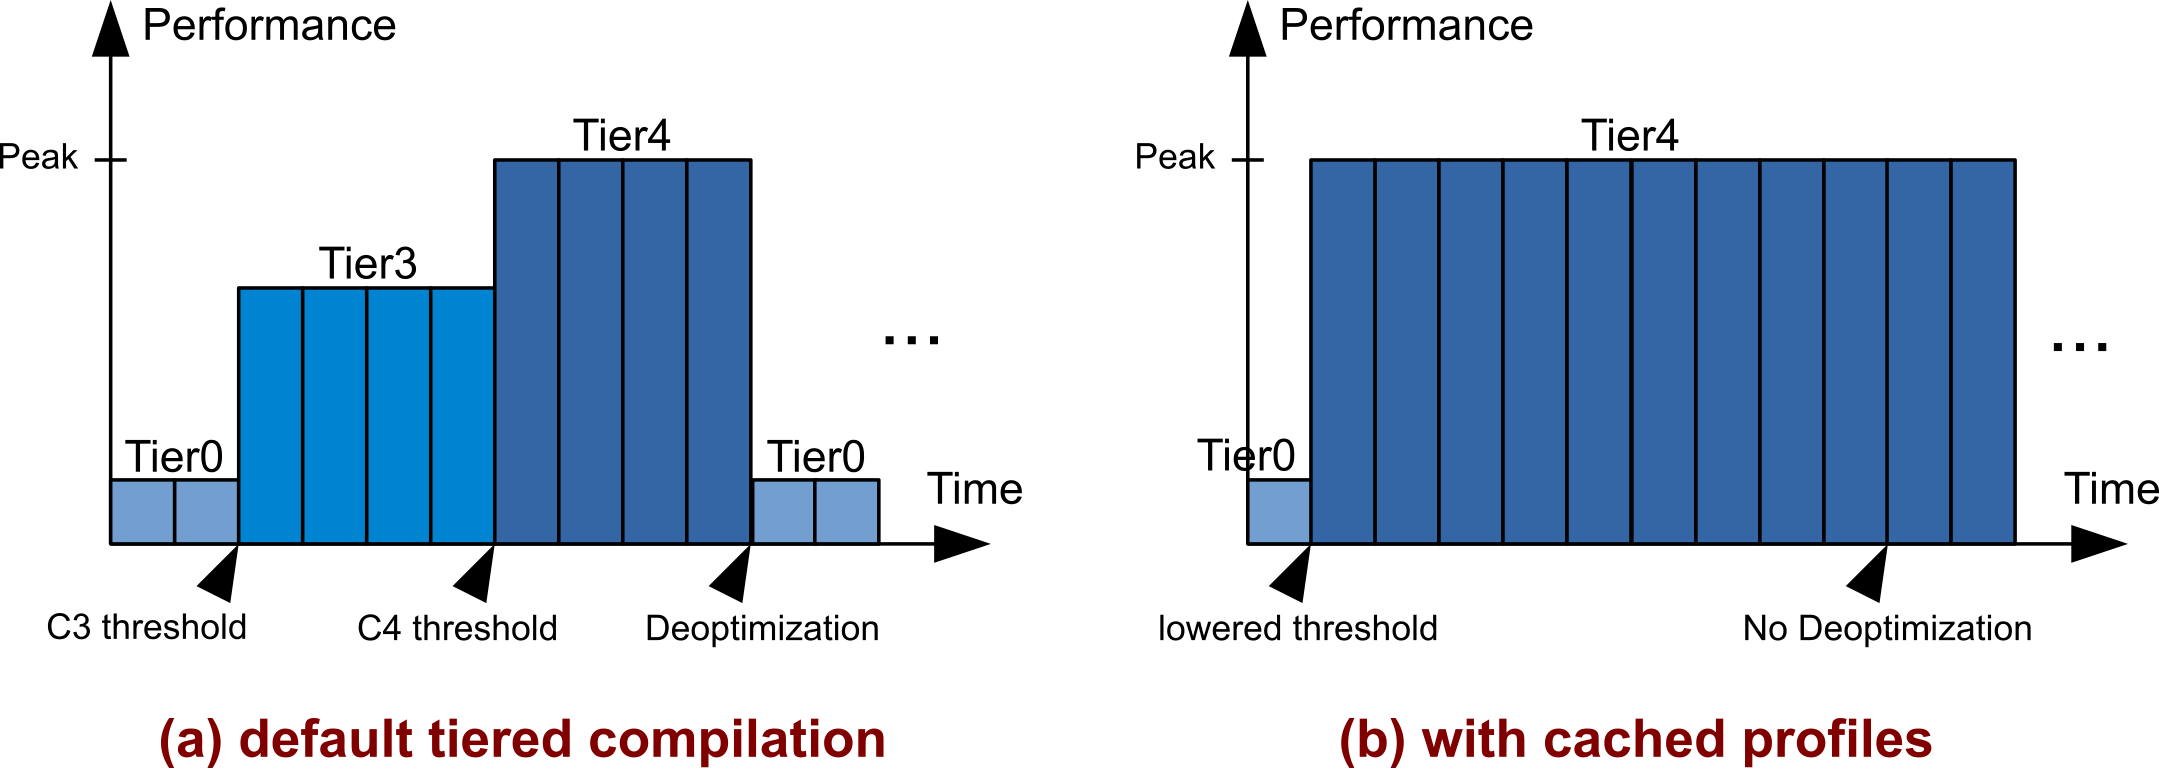
\includegraphics[width=0.9\textwidth]{figures/baseline_vs_usage.png}
    \caption{schematic visualization of cached profile benefit}
    \label{f:baseline_vs_usage}
  \end{center}
\end{figure}
Figure \ref{f:baseline_vs_usage} gives a schematic visualization of the expected effect on performance of a single method when using cached profiles compared to the current state without such a system and standard tiered compilation.
The blue bars roughly represent method invocations and higher bars equal higher compilation levels and therefore higher performance. The x-axis represents time since the start of the JVM. The figure shows the ideal case and abstracts away many details and other possible cases. However, it provides a good visualization for the examples provided in this chapter. A more detailed performance analysis, also considering worse cases is done in Chapter \ref{c:performance}.
\\\\
I'm using my implementation described in Chapter \ref{c:implementation} in CachedProfileMode 0 (see \ref{s:mode0}) built into openJDK 1.9.0.
All measurements in this chapter are done on a Dual-Core machine running at 2 GHz with 8GB of RAM. To measure the method invocation time I use hprof \cite{hprof} and the average of 10 runs. The evaluation process has been automated using a couple of python scripts. The error bars show the 95\% confidence interval.
\section{Example 1}
\label{s:ex1}
For this very first example, on-stack replacement has been disabled to keep the system simple and easy to understand.
\\
Example one is a simple class that invokes a method one hundred times. The method itself consists of a long running loop. The source code is shown in Listing \ref{l:nocompile}.
Since OSR is disabled and a compilation to level 3 is triggered after 200 invocations this method never leaves the interpreter. I call this run the \textit{Baseline}.
To show the influence of cached profiles I use a compiler flag to lower the compile threshold explicitly and, using the functionality written for this thesis, tell Hotspot to cache the profile.
In a next execution I use these profiles and achieve significantly better performance as one can see in Figure \ref{f:nocompile}.
This increase comes mainly from the fact that having a cached profile available allows the JVM to compile highly optimized code for hot methods earlier (at a lower threshold) since there is no need to gather the profiling information first.
\\
Since the example is rather simple neither the baseline nor the profile usage run trigger any deoptimization. This makes sense because after the first invocation, all the code paths of the method have been taken already and are therefore known to the interpreter and saved in the profile.
\begin{lstlisting}[float,caption=Simple method that does not get compiled,label=l:nocompile,language=Java]
class NoCompile {
    double result = 0.0;
    for(int c = 0; c < 100; c++) {
      result = method1(result);
    }
    public static double method1(double count) {
        for(int k = 0; k < 10000000; k++) {
            count = count + 50000;
        }
        return count;
   }
}
\end{lstlisting}
\begin{figure}[ht]
  \begin{center}
    \centering
    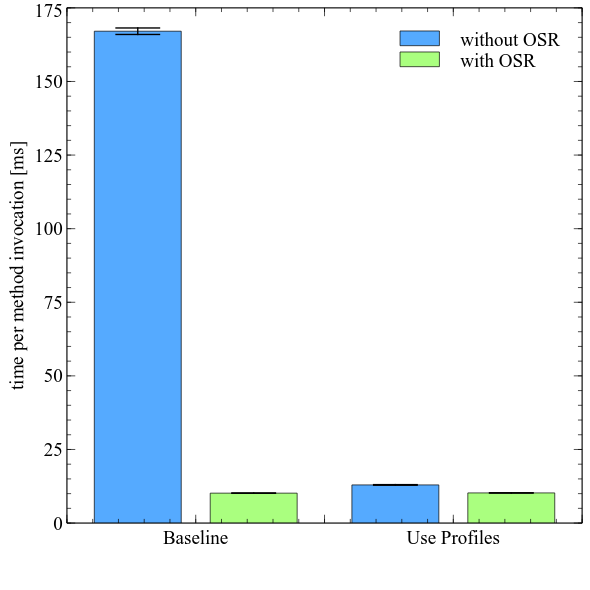
\includegraphics[width=0.5\textwidth]{figures/nocompile.png}
    \caption{NoCompile.method1 - per method invocation time}
    \label{f:nocompile}
  \end{center}
\end{figure}
\\
Enabling OSR again and the difference between with and without cached profiles vanishes.
This happens because Hotspot quickly realizes the hotness of the method and the JIT compiler produces perfectly optimized code during the first method invocation already. 
Even the OSR compiled code never triggers any deoptimization due to the simplicity of the loop.
So this example appears rather artificial since the same performance can be achieved with OSR already but nevertheless shows the influence of early compilation.
\section{Example 2}
\label{s:ex2}
However, OSR is one of the main features of Hotspot to improve the JIT performance and disabling that does not give us any practical results. Since we want an example which demonstrates the influence of cached profiles, I came up with the example sketched in Listing \ref{l:manydeopts} which is slightly more complex but still easy to understand.
\\\\
The idea is to create a method that takes a different, long running branch on each of it's method invocations. Each branch has been constructed in a way that it will trigger an OSR compilation. When compiling this method during its first iteration only the first branch will be included in the compiled code. The same will happen for each of the 100 method invocations. As one can see in Figure \ref{f:manydeopts} the baseline indeed averages at around 130 deoptimizations and a time per method invocation of 200 ms.
\\\\
Now I use a regular execution to dump the profiles and then use these profiles. So theoretically the profiles dumped after a full execution should include knowledge of all branches and therefore the compiled method using these profiles should not run into any deoptimizations. As one can see in Figure \ref{f:manydeopts} this is indeed the case. When using the cached profiles no more deoptimizations occur and because less time is spent profiling and compiling the methods the per method execution time is even significantly faster with averaging at 190ms now.
\begin{lstlisting}[float,caption=Simple method that causes many deoptimizations,label=l:manydeopts,language=Java]
class ManyDeopts {
    double result = 0.0;
    for(int c = 0; c < 100; c++) {
      result = method1(result);
    }
    public static long method1(long count) {
        for(int k = 0l; k < 10000000l; k++) {
            if (count < 10000000l) {
                count = count + 1;
            } else if (count < 30000000l) {
                count = count + 2;
                .
                .
                .
            } else if (count < 50500000000l) {
               count = count + 100;
            }
            count = count + 50000;
        }
        return count;
   }
}
\end{lstlisting}
\\\\\\\\\\\\
\begin{figure}[ht!]
  \begin{center}
    \centering
    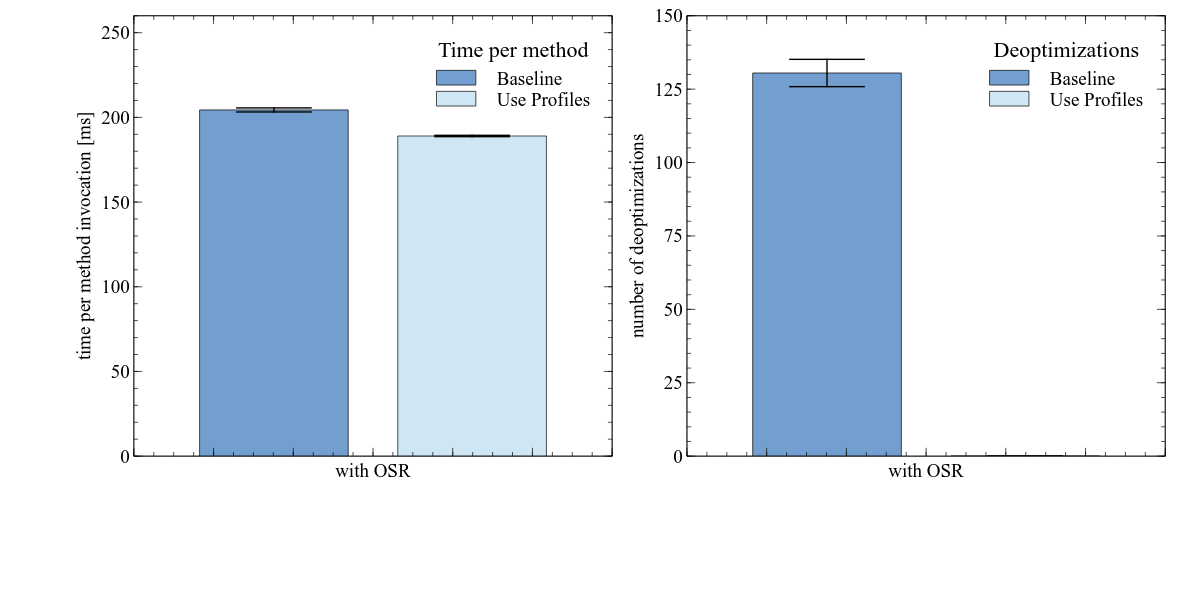
\includegraphics[width=0.9\textwidth]{figures/manydeopt.png}
    \caption{ManyDeopts.method1 - per method invocation time and deoptimization count}
    \label{f:manydeopts}
  \end{center}
\end{figure}
\\\\
\section{Similar systems}
\label{s:similarsystems}
In commercially available JVMs the idea of caching profiles is not new.
In fact the JVM developed and sold by Azul Systems\textregistered\ called Zing\textregistered\ \cite{zing} already offers a similar functionality.
Zing\textregistered\ includes a feature set they call ReadyNow!\texttrademark\ \cite{readynow} that aims to increase warmup performance of Java applications.
Their system has been designed with financial markets in mind and to overcome the issue of slow performance in the beginning and performance drops during execution.
Azul Systems clients reported that their production code usually experiences a significant performance drop as soon as the market goes live and the clients start trading.
The reasons are deoptimizations that occur because due to changed situation uncommon branch paths are taken or yet unused methods are invoked.
In the past their clients used techniques to warm up the JVM, for example doing fake trades. However this does not solve the problem since the JVM optimizes for these fake trades and still runs into deoptimizations once actual trades are meant to happen.
\\\\
ReadyNow!\texttrademark\  is a rich set of improvements how a JVM can overcome this issues. It includes attempts to reduce the number of deoptimizations in general and other not further specified optimizations.
As one of the core features Azul Systems\textregistered\ implemented the ability to log optimization statistics and decisions and reuse this logs in future runs. This is similar to the approach presented in this thesis. However they do not record the actual optimization but the learning and the reasons why certain optimizations happen. This gives them the ability to give feedback to the user of the JVM whether or not certain optimizations have been applied. They also provide APIs for developers to interact with the system and allow further fine-grained custom-designed optimizations.
\\\\
Unfortunately, they do not provide any numbers how their system actually improves performance.


\chapter{Implementation / Design}
\label{c:implementation}
This chapter describes the implementation of the cached profiles implementation for Hotspot, written as part of this thesis.
\\\\
Hotspot is an Java virtual machine implementation maintained by Oracle Cooperation. It is part of the open source project \texttt{OpenJDK} and the source code is available at \url{http://openjdk.java.net/}.
\\\\
Most of the work is included in two new classes \texttt{/share/vm/ci/ciCacheProfiles.cpp} and \\\texttt{/share/vm/ci/ciCacheProfilesBroker.cpp} as well as modifications to \texttt{/share/vm/ci/ciEnv.cpp} and \texttt{/share/vm/compiler/compileBroker.cpp}.
\\
Most of the code is located in \texttt{/share/vm/ci/ciCacheProfiles.cpp}, a class that takes care of setting up a datastructure for the cached profiles as well as providing public methods to check if a method is cached or not. The class \texttt{/share/vm/ci/ciCacheProfilesBroker.cpp} gets called before a method that has a profile available gets compiled. It is responsible for setting up the compilation environment so the JIT compiler can use the cached profiles.
\\\\
A full list of modified files and the changes can be seen in the webrev or appendix TODO.
\\\\
The changes are provided in form of a patch for Hotspot version 8182 TODO. This original version is referred to as \textit{Baseline}.
\\\\
I will describe and explain the functionality and the implementation design decision in the following sections, ordered by the appearance in execution.


\section{Creating cached profiles}
\label{s:creatingprofiles}
The baseline version of Hotspot already offered a functionality to replay a compilation based on dumped profiling information.
This is mainly used in case the JVM crashes during JIT compilation to replay the compilation again and help finding the cause of this crash.
Dumping the data needed for the replay is either be done automatically in case of a crash or can be invoked manually by specifying the \texttt{DumpReplay} compile command option per method.
I introduce method option called \texttt{DumpProfile} as well as a compiler flag \texttt{-XX:+DumpProfiles} that appends profiling information to a file as soon as the method gets compiled. The first option can be specified as part of the \texttt{-XX:CompileCommand} or \texttt{-XX:CompileCommandFile} flag and allows one to force single methods to dump their profile. The second commands dumps all profiles of all compiled methods into a single file called \textit{cached\_profiles.dat}.
\\\\
As soon as a method gets compiled all information about the methods used in the compiled method as well as their profiling information get converted to a string and written to disk. Since method often get compiled multiple times this can result in dumping compilation information about the same method multiple times. How this will be taken care of is described in Section \ref{s:initializingprofiles}
Together with some additional information about the compilation itself, for example the bytecode index of the compiled method in case of OSR, the compiler will be able to redo the same compilation on a future run of the java virtual machine.  
\section{Initializing cached profiles}
\label{s:initializingprofiles}
I introduce a new compiler flag \texttt{-XX:+CacheProfiles} that enables the use of profiles that have been written to disk in a previous run of the Java Virtual Machine. Per default it reads from a file called \textit{cached\_profiles.dat} but a different file can be specified using \\\texttt{-XX:CacheProfilesFile=other\_file.dat}.
\\\\
Before any cached profiles can be used the virtual machine has to parse that file and organize the profiles and compile information in a simple datastructure. This datastructure is kept in memory during the whole execution of the JVM to avoid multiple scans of the file.
The parsing process gets invoked during boot up of the JVM, directly after the compileBroker gets initialized. This happens before any methods get executed and blocks the JVM until finished.
As mentioned in Section \ref{s:creatingprofiles} the file consists of method informations, method profiles and additional compile information. The parser scans the file once and creates a so called \texttt{CompileRecord} for each of the methods that include compilation information in the file. This compile record also includes the list of method information and their profiling information.
A method's compile information could have been dumped multiple times, so it can happen that there are multiple CompileRecords for the same method. In this case, Hotspot will only keep the CompileRecords that are created based on the data written to the file last.
Since profiling information only grow, the compilation that happened last contains the richest profile and is considered the best to avoid deoptimizations.
\\\\
The CompileRecord as well as the lists of methods information and profiles are implemented as an array located in Hotspot's heap space.
They get initialized with a length of 8 and grow when needed. The choice has been done for simplicity and leaves up room for further optimizations.

\section{Using cached profiles}
\label{s:usingprofiles}
The idea is to use cached profiles whenever possible and if none are available continue as usual.
A graphical, simplified overview of the program flow for compiling a method with the changes introduced in this thesis can be found in Figure \ref{f:programflow}.
\begin{figure}[h]
  \begin{center}
    \centering
    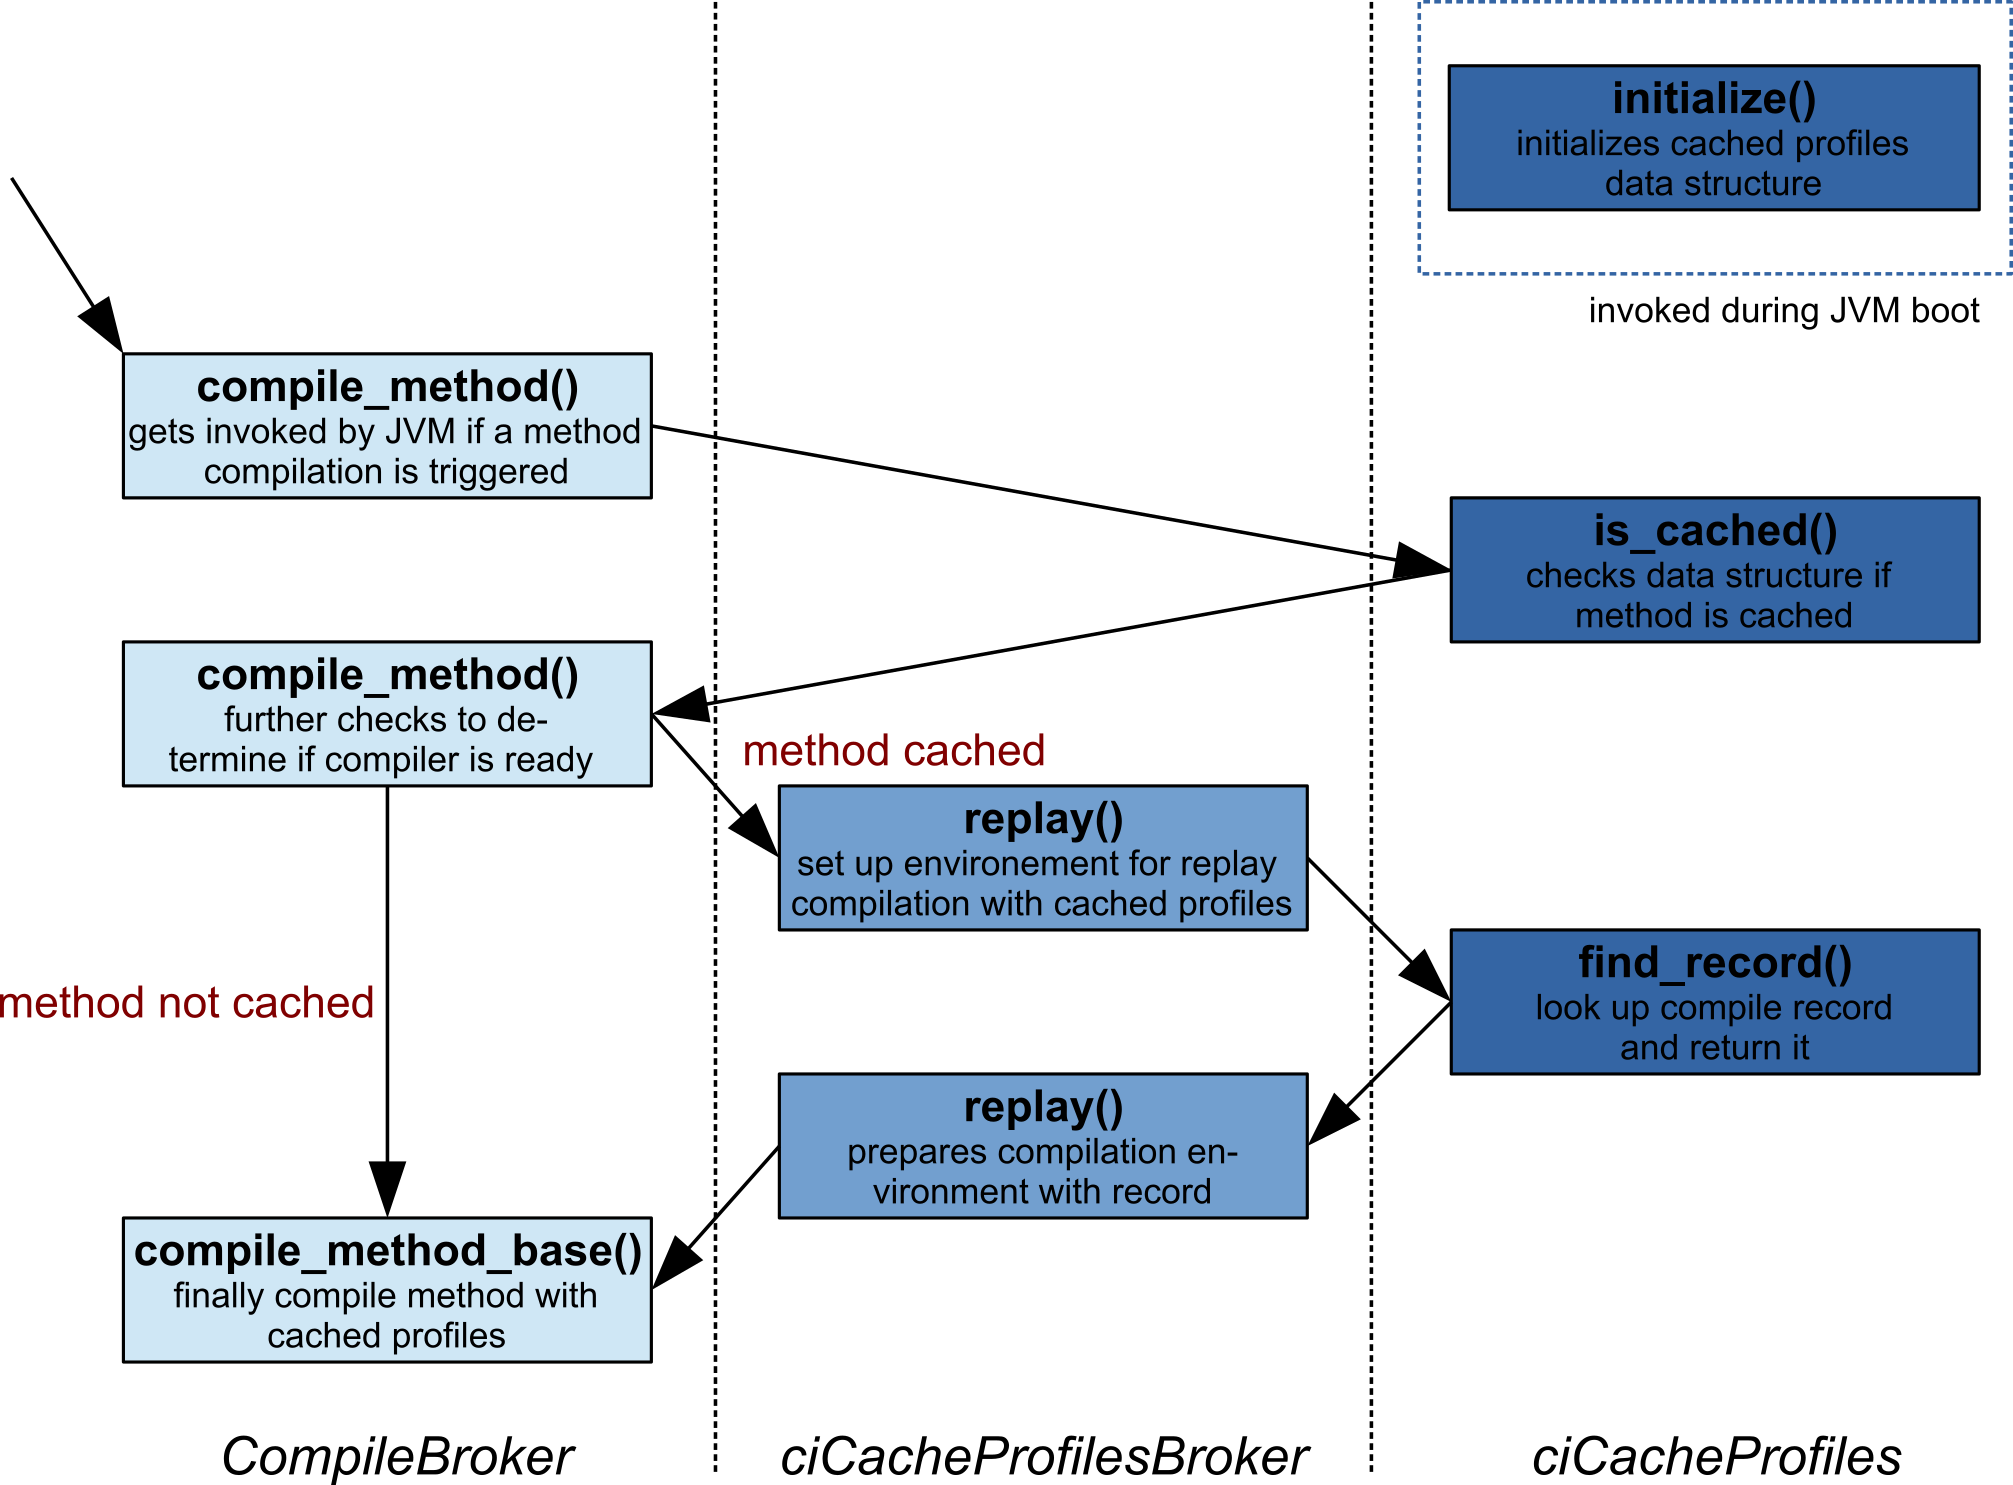
\includegraphics[width=0.8\textwidth]{figures/program_flow.png}
    \caption{program flow for compiling a method}
    \label{f:programflow}
  \end{center}
\end{figure}
As mentioned before once certain thresholds are exceeded a method gets scheduled for compilation. This means that the JVM will invoke a method called \texttt{compile\_method()} located in the \texttt{compileBroker} class. This method for example checks if the compile queue isn't full or if there is already another compilation of that particular method running.
I extended this method with a call to \texttt{ciCacheProfiles::is\_cached(Method* method)} which either returns 0 if the method is not cached or returns an integer value, reflecting the compile level, in case that method has a cached profile available.
In case the method is not cached the execution continues as in the baseline.
Otherwise the compileBroker will call into \texttt{ciCacheProfilesBroker} to replay the compilation, based on the saved profile.

\section{Different usage modes for cached profiles}
The implementation of cached profiles offers 3 different modes how
\label{s:cacheprofilesmode}
\subsection{Compile Thresholds lowered (mode 0)}
\label{s:mode0}
\subsection{Unmodified Compile Thresholds (mode 1)}
\label{s:mode1}
\subsection{Modified C1 stage (mode 2)}
\label{s:mode2}

\section{Debug outout}
\label{s:debugoutput}
For debugging and benchmarking purposes I implemented four debug flags that can be used along with \texttt{-XX:+CacheProfiles}.
-XX:+PrintCacheProfiles
-XX:+PrintDeoptimizationCount
-XX:+PrintDeoptimizationCountVerbose
-XX:+PrintCompileQueue


\chapter{Performance}
\label{c:performance}
\section{Examples}

\section{SPECjvm 2008}

\section{Nashorn / Octane}


\chapter{Possible Improvements}
\label{c:improvements}
- Better datasctructure
- Merging multiple profiles cleverly


\chapter{Conclusion}
\label{c:conclusion}
Modern Java Virtual Machines (JVM) like HotSpot gather profiling information about executed methods to improve the quality of the compiled code.
This thesis presents several approaches to reuse profiling information, that has been dumped to disk in previous executions of the JVM.
\\\\
The expected advantage is a faster warmup of the Java Virtual Machine, because the JVM does not need to spend time profiling the code and can use cached profiles directly.
Furthermore, since the cached profiles originate from previous compilations, where extensive profiling already happened, compilations using these profiles produce more optimized code, which decreases the amount of deoptimizations.
\\\\
We show, using two benchmark suites, that cached profiles can indeed improve warmup performance and significantly lower the amount of deoptimizations as well as reduce the time spent in the JIT compilers.
Therefore, we believe that cached profiles are a valuable asset in scenarios where a fast JVM warmup is needed and performance fluctuations at runtime should be avoided.
\\\\
In addition, we evaluated the performance of our approach with individual benchmarks for the impact of cached profiles on the load of the compile queue and the amount and type of compilations. The results show, that neither of them gives one-to-one correspondence between the examined factor and performance. However, the results provide indications, where the performance increase or decrease could come from.
\\\\
The functionality is implemented in the HotSpot JVM (OpenJDK9). Several new HotSpot options are added to allow fine tuning of the system, including the possibility to selectively enable or disable profile caching.

% -------------------------------------------------------------------------------------------------
% Appendices (if needed)
% -------------------------------------------------------------------------------------------------
\appendix
\chapter{Appendix}
\label{c:appendix}
\newpage
\section{Tiered compilation thresholds}
\label{a:compilethresholds}
\begin{table}[h]
  \centering
 % \caption{}
  \label{t:compilethresholds}
  \begin{center}
    \begin{tabular}{| l | p{9.0cm} | r | }
       \hline
       \textbf{flag} & \textbf{description} & \textbf{default} \\ \hline\hline
       CompileThresholdScaling & number of interpreted method invocations before (re-)compiling & 1.0\\ \hline
       Tier0InvokeNotifyFreqLog & Interpreter (tier 0) invocation notification frequency & 7\\ \hline
       Tier2InvokeNotifyFreqLog & C1 without MDO (tier 2) invocation notification frequency & 11 \\ \hline
       Tier3InvokeNotifyFreqLog & C1 with MDO profiling (tier 3) invocation notification frequency & 10 \\ \hline
       Tier23InlineeNotifyFreqLog & Inlinee invocation (tiers 2 and 3) notification frequency & 20 \\ \hline
       Tier0BackedgeNotifyFreqLog & Interpreter (tier 0) invocation notification frequency & 10 \\ \hline
       Tier2BackedgeNotifyFreqLog & C1 without MDO (tier 2) invocation notification frequency & 14 \\ \hline
       Tier3BackedgeNotifyFreqLog & C1 with MDO profiling (tier 3) invocation notification frequency & 13 \\ \hline
       Tier2CompileThreshold & threshold at which tier 2 compilation is invoked & 0 \\ \hline
       Tier2BackEdgeThreshold & Back edge threshold at which tier 2 compilation is invoked & 0 \\ \hline
       Tier3InvocationThreshold & Compile if number of method invocations crosses this threshold & 200 \\ \hline
       Tier3MinInvocationThreshold & Minimum invocation to compile at tier 3 & 100 \\ \hline
       Tier3CompileThreshold & Threshold at which tier 3 compilation is invoked (invocation minimum must be satisfied) & 2000 \\ \hline
       Tier3BackEdgeThreshold & Back edge threshold at which tier 3 OSR compilation is invoked & 60000 \\ \hline
       Tier4InvocationThreshold & Compile if number of method invocations crosses this threshold & 5000 \\ \hline
       Tier4MinInvocationThreshold & Minimum invocation to compile at tier 4 & 600 \\ \hline
       Tier4CompileThreshold & Threshold at which tier 4 compilation is invoked (invocation minimum must be satisfied) & 15000 \\ \hline
       Tier4BackEdgeThreshold & Back edge threshold at which tier 4 OSR compilation is invoked & 40000 \\ \hline
    \end{tabular}
  \end{center}
\end{table}
\newpage
\section{Cached profile example}
\label{a:cacheprofileexample}
\begin{lstlisting}[caption=Example of cached profiling information,label=l:cacheprofileexample,language=Java]
# 189 ciObject found
ciMethod java/lang/Double toString (D)Ljava/lang/String; 25 1 7 0 0
ciMethod java/lang/Long toString (J)Ljava/lang/String; 9 1 3 0 0
ciMethod java/lang/Long valueOf (J)Ljava/lang/Long; 25 1 7 0 0
ciMethod java/lang/Long longValue ()J 9 1 3 0 -1
ciMethodData java/lang/Double toString (D)Ljava/lang/String; 1 7 orig 280 152 101 83 95 3 127 0 0 88 140 138 72 3 127 0 0 144 1 0 0 0 0 0 0 0 0 0 0 0 0 0 0 0 0 0 0 0 0 0 0 0 0 0 0 0 0 0 0 0 0 0 0 0 0 0 0 0 0 0 0 0 0 0 0 0 0 0 0 0 0 0 0 0 0 0 0 0 0 0 0 77 68 79 32 101 120 116 114 97 32 100 97 116 97 32 108 111 99 107 0 0 0 0 0 0 0 0 0 0 0 0 0 0 0 0 0 0 0 0 0 0 0 0 0 0 0 0 0 0 0 0 0 0 0 0 0 0 0 0 0 0 0 0 0 0 0 0 0 0 0 0 0 0 0 0 0 0 0 0 0 0 0 0 0 0 0 0 0 0 0 0 0 0 0 0 0 0 0 0 0 0 0 0 0 0 0 0 0 0 0 0 0 0 0 0 0 0 0 0 0 0 0 0 0 0 0 0 0 0 0 0 0 0 0 0 0 3 0 0 0 33 0 0 0 1 0 0 0 0 0 0 0 0 0 0 0 0 0 0 0 248 3 0 0 248 31 0 0 2 0 0 0 0 0 0 0 0 0 0 0 48 0 0 0 254 255 255 255 0 0 0 0 2 0 4 0 0 0 0 0 data 16 0x40002 0x4 0x80002 0x4 0xf0002 0x4 0x0 0x0 0x0 0x0 0x0 0x0 0x9 0x2 0x0 0x0 oops 0 methods 0
ciMethodData java/lang/Long toString (J)Ljava/lang/String; 1 3 orig 280 152 101 83 95 3 127 0 0 248 47 139 72 3 127 0 0 40 2 0 0 136 0 0 0 0 0 0 0 0 0 0 0 0 0 0 0 0 0 0 0 0 0 0 0 0 0 0 0 0 0 0 0 0 0 0 0 0 0 0 0 0 0 0 0 0 0 0 0 0 0 0 0 0 0 0 0 0 0 0 0 77 68 79 32 101 120 116 114 97 32 100 97 116 97 32 108 111 99 107 0 0 0 0 0 0 0 0 0 0 0 0 0 0 0 0 0 0 0 0 0 0 0 0 0 0 0 0 0 0 0 0 0 0 0 0 0 0 0 0 0 0 0 0 0 0 0 0 0 0 0 0 0 0 0 0 0 0 0 0 0 0 0 0 0 0 0 0 0 0 0 0 0 0 0 0 0 0 0 0 0 0 0 0 0 0 0 0 0 0 0 0 0 0 0 0 0 0 0 0 0 0 0 0 0 0 0 0 0 0 0 0 0 0 0 0 0 1 0 0 0 17 0 0 0 1 0 0 0 0 0 0 0 0 0 0 0 0 0 0 0 248 3 0 0 248 31 0 0 2 0 0 0 0 0 0 0 0 0 0 0 200 0 0 0 254 255 255 255 0 0 0 0 2 0 5 0 0 0 0 0 data 35 0x50002 0x2 0xd0007 0x2 0x30 0x0 0x170002 0x0 0x1e0007 0x2 0x48 0x0 0x230002 0x0 0x280003 0x0 0x28 0x2c0002 0x2 0x370002 0x2 0x400002 0x2 0x480002 0x2 0x0 0x0 0x0 0x0 0x0 0x0 0x9 0x2 0x0 0x0 oops 0 methods 0
ciMethodData java/lang/Long valueOf (J)Ljava/lang/Long; 1 7 orig 280 152 101 83 95 3 127 0 0 232 61 139 72 3 127 0 0 224 1 0 0 80 0 0 0 0 0 0 0 0 0 0 0 0 0 0 0 0 0 0 0 0 0 0 0 0 0 0 0 0 0 0 0 0 0 0 0 0 0 0 0 0 0 0 0 0 0 0 0 0 0 0 0 0 0 0 0 0 0 0 0 77 68 79 32 101 120 116 114 97 32 100 97 116 97 32 108 111 99 107 0 0 0 0 0 0 0 0 0 0 0 0 0 0 0 0 0 0 0 0 0 0 0 0 0 0 0 0 0 0 0 0 0 0 0 0 0 0 0 0 0 0 0 0 0 0 0 0 0 0 0 0 0 0 0 0 0 0 0 0 0 0 0 0 0 0 0 0 0 0 0 0 0 0 0 0 0 0 0 0 0 0 0 0 0 0 0 0 0 0 0 0 0 0 0 0 0 0 0 0 0 0 0 0 0 0 0 0 0 0 0 0 0 0 0 0 0 3 0 0 0 33 0 0 0 1 0 0 0 0 0 0 0 0 0 0 0 0 0 0 0 248 3 0 0 248 31 0 0 2 0 0 0 0 0 0 0 0 0 0 0 128 0 0 0 254 255 255 255 0 0 0 0 2 0 5 0 0 0 0 0 data 26 0x50002 0x4 0xd0007 0x0 0x50 0x4 0x150007 0x4 0x30 0x0 0x270002 0x0 0x300002 0x4 0x380002 0x4 0x0 0x0 0x0 0x0 0x0 0x0 0x9 0x2 0x0 0x0 oops 0 methods 0
ciMethodData java/lang/Long longValue ()J 1 3 orig 280 152 101 83 95 3 127 0 0 176 67 139 72 3 127 0 0 120 1 0 0 0 0 0 0 0 0 0 0 0 0 0 0 0 0 0 0 0 0 0 0 0 0 0 0 0 0 0 0 0 0 0 0 0 0 0 0 0 0 0 0 0 0 0 0 0 0 0 0 0 0 0 0 0 0 0 0 0 0 0 0 77 68 79 32 101 120 116 114 97 32 100 97 116 97 32 108 111 99 107 0 0 0 0 0 0 0 0 0 0 0 0 0 0 0 0 0 0 0 0 0 0 0 0 0 0 0 0 0 0 0 0 0 0 0 0 0 0 0 0 0 0 0 0 0 0 0 0 0 0 0 0 0 0 0 0 0 0 0 0 0 0 0 0 0 0 0 0 0 0 0 0 0 0 0 0 0 0 0 0 0 0 0 0 0 0 0 0 0 0 0 0 0 0 0 0 0 0 0 0 0 0 0 0 0 0 0 0 0 0 0 0 0 0 0 0 0 1 0 0 0 17 0 0 0 1 0 0 0 0 0 0 0 0 0 0 0 0 0 0 0 248 3 0 0 248 31 0 0 2 0 0 0 0 0 0 0 0 0 0 0 32 0 0 0 254 255 255 255 0 0 0 0 2 0 5 0 0 0 0 0 data 13 0x50002 0x2 0x110002 0x2 0x0 0x0 0x0 0x0 0x0 0x0 0x9 0x1 0x0 oops 0 methods 0
ciMethod NoCompile method1 (D)D 17 80000001 4 0 -1
ciMethodData NoCompile method1 (D)D 2 30002544 orig 280 152 101 83 95 3 127 0 0 200 8 192 72 3 127 0 0 40 5 0 0 112 1 0 0 0 0 0 0 0 0 0 0 0 0 0 0 0 0 0 0 0 0 0 0 0 0 0 0 0 0 0 0 0 0 0 0 0 0 0 0 0 0 0 0 0 0 0 0 0 0 0 0 0 0 0 0 0 0 0 0 77 68 79 32 101 120 116 114 97 32 100 97 116 97 32 108 111 99 107 0 0 0 0 0 0 0 0 0 0 0 0 0 0 0 0 0 0 0 0 0 0 0 0 0 0 0 0 0 0 0 0 0 0 0 0 0 0 0 0 0 0 0 0 0 0 0 0 0 0 0 0 0 0 0 0 0 0 0 0 0 0 0 0 0 0 0 0 0 0 0 0 0 0 0 0 0 0 0 0 0 0 0 0 0 0 0 0 0 0 0 0 0 0 0 0 0 0 0 0 0 0 0 0 0 0 0 0 0 0 0 0 0 0 0 0 0 128 150 152 0 17 0 0 0 193 170 137 9 0 0 0 0 0 0 0 0 0 0 0 0 0 0 0 0 56 0 0 0 2 0 0 0 1 0 12 0 2 0 0 0 200 3 0 0 254 255 255 255 0 0 0 0 2 0 4 0 0 0 0 0 data 131 0x40002 0x2 0xa0007 0x0 0x130 0x2 0x140002 0x2 0x190005 0x0 0x7f03580bbc90 0x2 0x0 0x0 0x1d0002 0x2 0x200005 0x0 0x7f03580bbc90 0x2 0x0 0x0 0x250005 0x0 0x7f03580bbc90 0x2 0x0 0x0 0x280005 0x0 0x7f03580bbc90 0x2 0x0 0x0 0x2b0005 0x0 0x7f031402b870 0x2 0x0 0x0 0x2e0002 0x2 0x390007 0x1 0x38 0x989edd 0x450003 0x989edc 0xffffffffffffffe0 0x480002 0x1 0x500007 0x0 0x1a0 0x1 0x5a0002 0x1 0x5f0005 0x1 0x0 0x0 0x0 0x0 0x6a0002 0x1 0x6d0005 0x1 0x0 0x0 0x0 0x0 0x720005 0x1 0x0 0x0 0x0 0x0 0x760002 0x1 0x790005 0x1 0x0 0x0 0x0 0x0 0x7e0005 0x1 0x0 0x0 0x0 0x0 0x810005 0x1 0x0 0x0 0x0 0x0 0x840005 0x0 0x7f031402b870 0x1 0x0 0x0 0x8c0002 0x1 0x8f0005 0x1 0x0 0x0 0x0 0x0 0x940002 0x1 0x970005 0x0 0x7f031402b920 0x1 0x0 0x0 0xa20002 0x1 0x0 0x0 0x0 0x0 0x0 0x0 0x9 0x2 0x0 0x0 oops 7 10 java/lang/StringBuilder 18 java/lang/StringBuilder 24 java/lang/StringBuilder 30 java/lang/StringBuilder 36 java/io/PrintStream 99 java/io/PrintStream 115 java/util/ArrayList methods 0
compile NoCompile method1 (D)D -1 4 inline 24 0 -1 NoCompile method1 (D)D 1 20 java/lang/StringBuilder <init> ()V 2 10 java/lang/AbstractStringBuilder <init> (I)V 3 8 java/lang/Object <init> ()V 1 25 java/lang/StringBuilder append (Ljava/lang/String;)Ljava/lang/StringBuilder; 1 32 java/lang/StringBuilder append (Ljava/lang/String;)Ljava/lang/StringBuilder; 1 37 java/lang/StringBuilder append (Ljava/lang/String;)Ljava/lang/StringBuilder; 1 90 java/lang/StringBuilder <init> ()V 2 10 java/lang/AbstractStringBuilder <init> (I)V 3 8 java/lang/Object <init> ()V 1 95 java/lang/StringBuilder append (Ljava/lang/String;)Ljava/lang/StringBuilder; 1 109 java/lang/StringBuilder append (Ljava/lang/String;)Ljava/lang/StringBuilder; 1 114 java/lang/StringBuilder append (Ljava/lang/String;)Ljava/lang/StringBuilder; 1 121 java/lang/StringBuilder append (Ljava/lang/String;)Ljava/lang/StringBuilder; 1 126 java/lang/StringBuilder append (Ljava/lang/String;)Ljava/lang/StringBuilder; 1 140 java/lang/Long valueOf (J)Ljava/lang/Long; 2 48 java/lang/Long <init> (J)V 3 9 java/lang/Number <init> ()V 4 7 java/lang/Object <init> ()V 1 143 java/lang/Long longValue ()J 1 148 java/lang/Long valueOf (J)Ljava/lang/Long; 2 48 java/lang/Long <init> (J)V 3 9 java/lang/Number <init> ()V 4 7 java/lang/Object <init> ()V
\end{lstlisting}

\section{Code changes}
\label{a:codechanges}
\begin{table}[ht!]
  \caption{Code lines changed, inserted, deleted, modified and unchanged}
  \label{t:codechanges}
  \begin{center}
    \begin{tabular}{|l|c|c|c|c|c|}
    \hline
      class (in src/share/vm/) & changed & inserted & deleted & modified & unchg. \\ \hline
      ci/c1\_Compilation.cpp & 6 & 6 & 0 & 0 & 708\\ \hline
      ci/ciClassList.hpp & 2 & 2 & 0 & 0 & 121\\ \hline
      ci/ciEnv.cpp & 58 & 56 & 0 & 2 & 1283 \\ \hline
      ci/ciEnv.hpp & 5 & 5 & 0 & 0 & 469 \\ \hline
      ci/ciMethod.cpp & 4 & 4 & 0 & 0 & 1480 \\ \hline
      ci/ciMethod.hpp & 1 & 1 & 0 & 0 & 350 \\ \hline
      ci/ciMethodData.cpp & 4 & 4 & 0 & 0 & 797 \\ \hline
      ci/ciMethodData.hpp & 1 & 1 & 0 & 0 & 595 \\ \hline
      compiler/compileBroker.cpp & 78 & 77 & 1 & 0 & 2401 \\ \hline
      compiler/compileBroker.hpp & 2 & 2 & 0 & 0 & 478 \\ \hline
      interpreter/invocationCounter.hpp & 2 & 2 & 0 & 0 & 156 \\ \hline
      oops/instanceKlass.hpp & 2 & 2 & 0 & 0 & 1383 \\ \hline
      oops/methodCounters.cpp & 14 & 13 & 1 & 0 & 74 \\ \hline
      oops/methodCounters.hpp & 4 & 4 & 0 & 0 & 208 \\ \hline
      oops/methodData.cpp & 9 & 9 & 0 & 0 & 1686 \\ \hline
      opto/compile.cpp & 9 & 9 & 0 & 0 & 4418 \\ \hline
      prims/jvmtiExport.hpp & 2 & 2 & 0 & 0 & 542 \\ \hline 
      runtime/advancedThresholdPolicy.cpp & 5 & 5 & 0 & 0 & 537 \\ \hline
      runtime/deoptimization.cpp & 15 & 15 & 0 & 0 & 2043 \\ \hline
      runtime/deoptimization.hpp & 7 & 7 & 0 & 0 & 407 \\ \hline
      runtime/globals.hpp & 41 & 38 & 0 & 3 & 3967 \\ \hline
      runtime/java.cpp & 8 & 8 & 0 & 0 & 744 \\ \hline
      runtime/simpleThresholdPolicy.inline.hpp & 51 & 49 & 0 & 2 & 80 \\ \hline
      /runtime/thread.cpp & 7 & 7 & 0 & 0 & 4585 \\ \hline  
      /ci/ciCacheProfiles.cpp & 801 & 801 & 0 & 0 & 0 \\ \hline  
      /ci/ciCacheProfiles.hpp & 337 & 337 & 0 & 0 & 0 \\ \hline 
      /ci/ciCacheProfilesBroker.cpp & 292 & 292 & 0 & 0 & 0 \\ \hline 
      /ci/ciCacheProfilesBroker.hpp & 79 & 79 & 0 & 0 & 0 \\ \hline 
    \end{tabular}
  \end{center}
\end{table}
\section{SPECjvm benchmark}
\label{a:specjvm_benchmark}
This list gives a short description of the benchmarks that are part of the SPECjvm 2008 Benchmark Suite.
The list is directly taken from \url{https://www.spec.org/jvm2008/docs/benchmarks/index.html} and put in as a reference.
\begin{itemize}
  \item \texttt{Compress: } This benchmark compresses data, using a modified Lempel-Ziv method (LZW). Basically finds common substrings and replaces them with a variable size code. This is deterministic, and can be done on the fly. Thus, the decompression procedure needs no input table, but tracks the way the table was built. Algorithm from "A Technique for High Performance Data Compression", Terry A. Welch, IEEE Computer Vol 17, No 6 (June 1984), pp 8-19.

This is a Java port of the 129.compress benchmark from CPU95, but improves upon that benchmark in that it compresses real data from files instead of synthetically generated data as in 129.compress. 
 \item \texttt{Crypto: } This benchmark focuses on different areas of crypto and are split in three different sub-benchmarks. The different benchmarks use the implementation inside the product and will therefore focus on both the vendor implementation of the protocol as well as how it is executed.
  \begin{itemize}
    \item \texttt{aes} encrypt and decrypt using the AES and DES protocols, using CBC/PKCS5Padding and CBC/NoPadding. Input data size is 100 bytes and 713 kB.
    \item \texttt{rsa} encrypt and decrypt using the RSA protocol, using input data of size 100 bytes and 16 kB.
    \item \texttt{signverify} sign and verify using MD5withRSA, SHA1withRSA, SHA1withDSA and SHA256withRSA protocols. Input data size of 1 kB, 65 kB and 1 MB.
  \end{itemize}
\item \texttt{Derby: } This benchmark uses an open-source database written in pure Java. It is synthesized with business logic to stress the BigDecimal library. It is a direct replacement to the SPECjvm98 db benchmark but is more capable and represents as close to a "real" application. The focus of this benchmark is on BigDecimal computations (based on telco benchmark) and database logic, especially, on locks behavior. BigDecimal computations are trying to be outside 64-bit to examine not only 'simple' BigDecimal, where 'long' is used often for internal representation. 
\item \texttt{MPEGaudio: } This benchmark is very similar to the SPECjvm98 mpegaudio. The mp3 library has been replaced with JLayer, an LGPL mp3 library. Its floating-point heavy and a good test of mp3 decoding. Input data were taken from SPECjvm98.
\item \texttt{Scimark: } This benchmark was developed by NIST and is widely used by the industry as a floating point benchmark. Each of the subtests (\texttt{fft, lu, monte\_carlo, sor, sparse}) were incorporated into SPECjvm2008. There are two versions of this test, one with a \"large\" dataset (32Mbytes) which stresses the memory subsystem and a \"small\" dataset which stresses the JVMs (512Kbytes).
\item \texttt{Serial: } This benchmark serializes and deserializes primitives and objects, using data from the JBoss benchmark. The benchmark has a producer-consumer scenario where serialized objects are sent via sockets and deserialized by a consumer on the same system. The benchmark heavily stress the Object.equals() test.
\item \texttt{Sunflow: } This benchmark tests graphics visualization using an open source, internally multi-threaded global illumination rendering system. The sunflow library is threaded internally, i.e. it's possible to run several bundles of dependent threads to render an image. The number of internal sunflow threads is required to be 4 for a compliant run. It is however possible to configure in property specjvm.benchmark.sunflow.threads.per.instance, but no more than 16, per sunflow design. Per default, the benchmark harness will use half the number of benchmark threads, i.e. will run as many sunflow benchmark instances in parallel as half the number of hardware threads. This can be configured in specjvm.benchmark.threads.sunflow.
\item \texttt{XML: } This benchmark has two sub-benchmarks: XML.transform and XML.validation.
\\XML.transform exercises the JRE's implementation of javax.xml.transform (and associated APIs) by applying style sheets (.xsl files) to XML documents. The style sheets and XML documents are several real life examples that vary in size (3KB to 156KB) and in the style sheet features that are used most heavily. One "operation" of XML.transform consists of processing each style sheet / document pair, accessing the XML document as a DOM source, a SAX source, and a Stream source. In order that each style sheet / document pair contribute about equally to the time taken for a single operation, some of the input pairs are processed multiple times during one operation.

Result verification for XML.transform is somewhat more complex than for other of the benchmarks because different XML style sheet processors can produce results that are slightly different from each other, but all still correct. In brief, the process used is this. First, before the measurement interval begins the workload is run once and the output is collected, canonicalized (per the specification of canonical XML form) and compared with the expected canonicalized output. Output from transforms that produce HTML is converted to XML before canonicalization. Also, a checksum is generated from this output. Inside the measurement interval the output from each operation is only checked using the checksum.

XML.validation exercises the JRE's implementation of javax.xml.validation (and associated APIs) by validating XML instance documents against XML schemata (.xsd files). The schemata and XML documents are several real life examples that vary in size (1KB to 607KB) and in the XML schema features that are used most heavily. One "operation" of XML.validation consists of processing each style sheet / document pair, accessing the XML document as a DOM source and a SAX source. As in XML.transform, some of the input pairs are processed multiple times during one operation so that each input pair contributes about equally to the time taken for a single operation. 
\end{itemize}

\section{Octane benchmark}
\label{a:octane_benchmark}
What follows is an overview of the benchmarks Octane consists of.
The original list can be found on \url{https://developers.google.com/octane/benchmark}.
\begin{itemize}
\item \texttt{Richards: }OS kernel simulation benchmark, originally written in BCPL by Martin Richards (539 lines).
  \begin{itemize}
    \item Main focus: \textit{property load/store, function/method calls}
    \item Secondary focus: \textit{code optimization, elimination of redundant code}
  \end{itemize}
\item \texttt{Deltablue: }One-way constraint solver, originally written in Smalltalk by John Maloney and Mario Wolczko (880 lines).
  \begin{itemize}
    \item Main focus: \textit{polymorphism}
    \item Secondary focus: \textit{OO-style programming}
  \end{itemize}
\item \texttt{Raytrace: }Ray tracer benchmark based on code by Adam Burmister (904 lines).
  \begin{itemize}
    \item Main focus: \textit{argument object, apply}
    \item Secondary focus: \textit{prototype library object, creation pattern}
  \end{itemize}
\item \texttt{Regexp: }Regular expression benchmark generated by extracting regular expression operations from 50 of the most popular web pages (1761 lines).
  \begin{itemize}
    \item Main focus: \textit{Regular expressions}
  \end{itemize}
  \item \texttt{NavierStokes: }2D NavierStokes equations solver, heavily manipulates double precision arrays. Based on Oliver Hunt's code (387 lines).
  \begin{itemize}
    \item Main focus: \textit{reading and writing numeric arrays.}
    \item Secondary focus: \textit{floating point math.}
  \end{itemize}
  \item \texttt{Crypto: }Encryption and decryption benchmark based on code by Tom Wu (1698 lines).
  \begin{itemize}
    \item Main focus: \textit{bit operations}
  \end{itemize}
  \item \texttt{Splay: }Data manipulation benchmark that deals with splay trees and exercises the automatic memory management subsystem (394 lines).
  \begin{itemize}
    \item Main focus: \textit{Fast object creation, destruction}
  \end{itemize}
 \item \texttt{SplayLatency: }The Splay test stresses the Garbage Collection subsystem of a VM. SplayLatency instruments the existing Splay code with frequent measurement checkpoints. A long pause between checkpoints is an indication of high latency in the GC. This test measures the frequency of latency pauses, classifies them into buckets and penalizes frequent long pauses with a low score.
  \begin{itemize}
    \item Main focus: \textit{Garbage Collection latency}
  \end{itemize}
  \item \texttt{EarleyBoyer: }Classic Scheme benchmarks, translated to JavaScript by Florian Loitsch's Scheme2Js compiler (4684 lines).
  \begin{itemize}
    \item Main focus: \textit{Fast object creation, destruction}
    \item Secondary focus: \textit{closures, arguments object}
  \end{itemize}
  \item \texttt{pdf.js: }Mozilla's PDF Reader implemented in JavaScript. It measures decoding and interpretation time (33,056 lines).
  \begin{itemize}
    \item Main focus: \textit{array and typed arrays manipulations.}
    \item Secondary focus: \textit{math and bit operations, support for future language features (e.g. promises)}
  \end{itemize}
  \item \texttt{Mandreel: }Runs the 3D Bullet Physics Engine ported from C++ to JavaScript via Mandreel (277,377 lines).
  \begin{itemize}
    \item Main focus: \textit{emulation}
  \end{itemize}
  \item \texttt{MandreelLatency: }Similar to the SplayLatency test, this test instruments the Mandreel benchmark with frequent time measurement checkpoints. Since Mandreel stresses the VM's compiler, this test provides an indication of the latency introduced by the compiler. Long pauses between measurement checkpoints lower the final score.
  \begin{itemize}
    \item Main focus: \textit{Compiler latency}
  \end{itemize}
  \item \texttt{GB Emulator: }Emulates the portable console's architecture and runs a demanding 3D simulation, all in JavaScript (11,097 lines).
  \begin{itemize}
    \item Main focus: \textit{emulation}
  \end{itemize}
    \item \texttt{Code loading: }Measures how quickly a JavaScript engine can start executing code after loading a large JavaScript program, social widget being a common example. The source for this test is derived from open source libraries (Closure, jQuery) (1,530 lines).
  \begin{itemize}
    \item Main focus: \textit{JavaScript parsing and compilation}
  \end{itemize}
    \item \texttt{Box2DWeb: }Based on Box2DWeb, the popular 2D physics engine originally written by Erin Catto, ported to JavaScript. (560 lines, 9000+ de-minified)
  \begin{itemize}
    \item Main focus: \textit{floating point math.}
    \item Secondary focus: \textit{properties containing doubles, accessor properties.}
  \end{itemize}
    \item \texttt{Typescript: }Microsoft's TypeScript compiler is a complex application. This test measures the time TypeScript takes to compile itself and is a proxy of how well a VM handles complex and sizable Javascript applications (25,918 lines).
  \begin{itemize}
    \item Main focus: \textit{run complex, heavy applications}
  \end{itemize}
\end{itemize}
\section{Additional graphs}
\label{a:additional_graphs}
% --------------------------- SPECjvm compress Queue ------------------
\begin{figure}[ht]
  \begin{center}
    \centering
    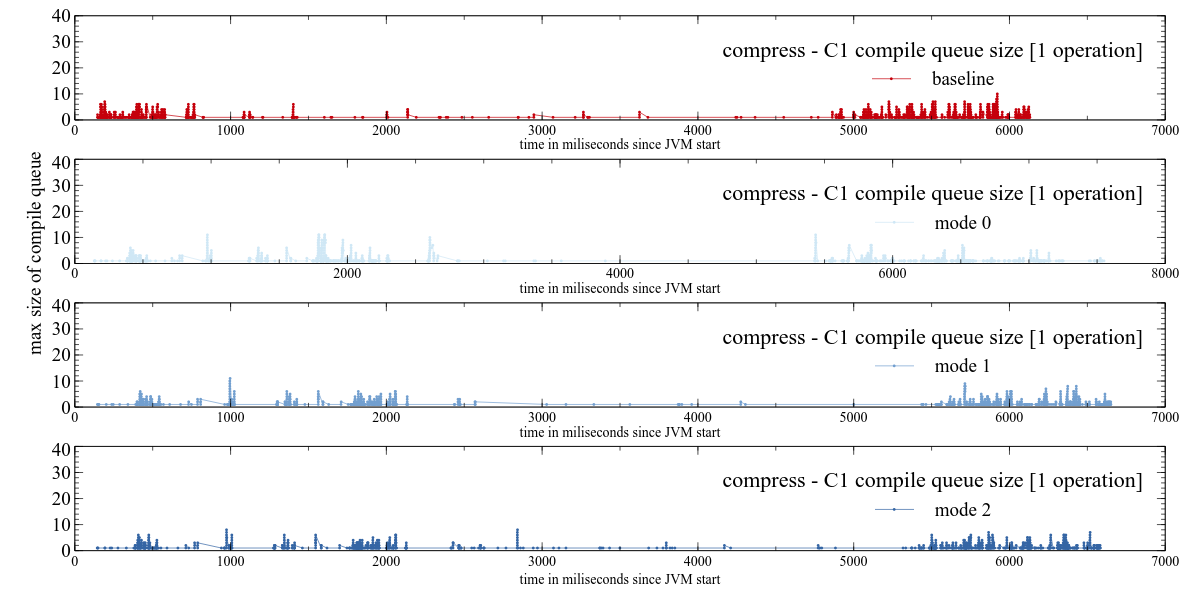
\includegraphics[width=1.0\textwidth]{figures/spec_queue_compress_separate_c1.png}
    \caption{C1 Compile queue size over time SPECjvm compress benchmark}
    \label{f:spec_queue_compress_separate_c1}
  \end{center}
\end{figure}
\begin{figure}[ht]
  \begin{center}
    \centering
    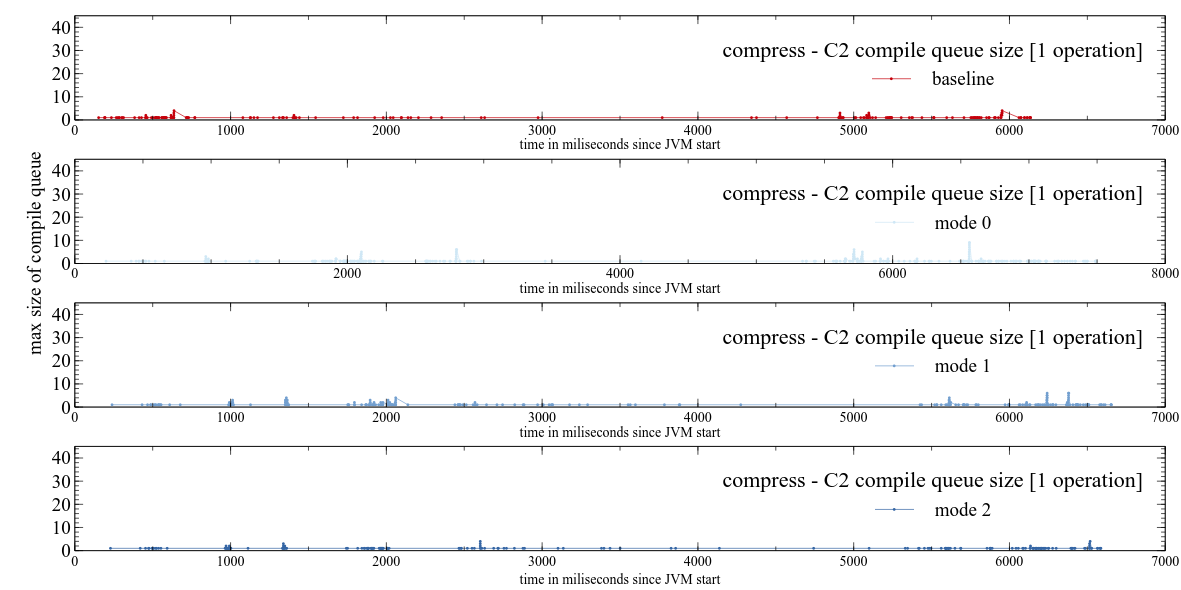
\includegraphics[width=1.0\textwidth]{figures/spec_queue_compress_separate_c2.png}
    \caption{C2 Compile queue size over time SPECjvm compress benchmark}
    \label{f:spec_queue_compress_separate_c2}
  \end{center}
\end{figure}
% --------------------------- SPECjvm scimark.sparse.large Queue ------------------
\begin{figure}[ht]
  \begin{center}
    \centering
    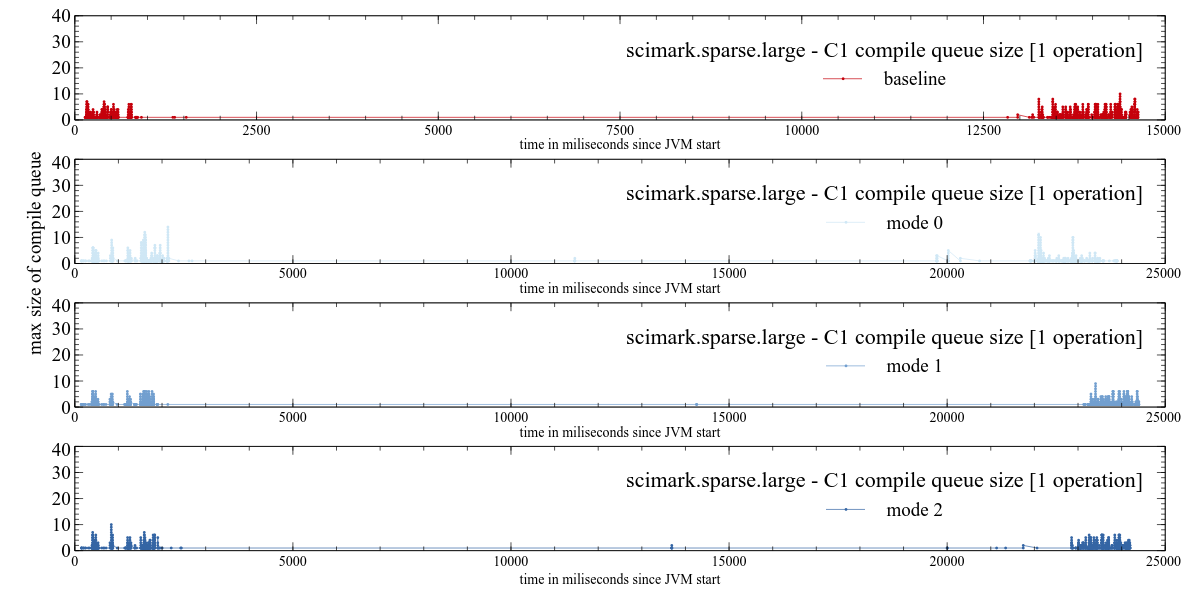
\includegraphics[width=1.0\textwidth]{figures/spec_queue_scirmarksparselarge_separate_c1.png}
    \caption{C1 Compile queue size over time SPECjvm scimark.sparse.large benchmark}
    \label{f:spec_queue_scirmarksparselarge_separate_c1}
  \end{center}
\end{figure}
\begin{figure}[ht]
  \begin{center}
    \centering
    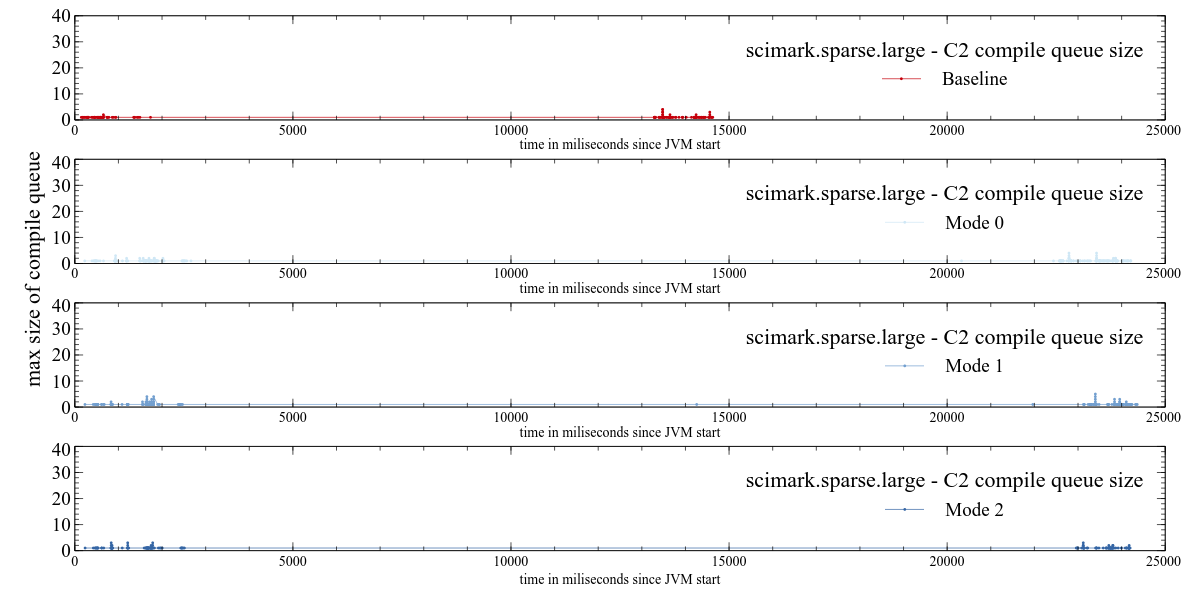
\includegraphics[width=1.0\textwidth]{figures/spec_queue_scirmarksparselarge_separate_c2.png}
    \caption{C2 Compile queue size over time SPECjvm scimark.sparse.large benchmark}
    \label{f:spec_queue_scirmarksparselarge_separate_c2}
  \end{center}
\end{figure}


% -------------------------------------------------------------------------------------------------
% Bibliography
% -------------------------------------------------------------------------------------------------
\addcontentsline{toc}{chapter}{Bibliography}
\bibliography{bibliography}

\end{document}
